% ============================================================================
% Homicides and Labor Market Conditions in Ecuador, 2018-2026:
% Descriptive and Quasi-Experimental Evidence from a Province-Quarter Panel
% ----------------------------------------------------------------------------
% arXiv submission package (econ.EM / econ.GN).
% Compile: pdflatex main.tex && bibtex main && pdflatex main.tex && pdflatex main.tex
% ============================================================================
\documentclass[11pt]{article}

\usepackage[utf8]{inputenc}
\usepackage[T1]{fontenc}
\usepackage{amsmath,amssymb}
\usepackage{graphicx}
\usepackage{booktabs}
\usepackage[margin=1in]{geometry}
\usepackage[hidelinks]{hyperref}
\usepackage{xcolor}

\graphicspath{{figures/}}

\title{\textbf{Homicides and Labor Market Conditions in Ecuador, 2018--2026: \\ Descriptive and Quasi-Experimental Evidence from a Province--Quarter Panel}}

% >>> AUTOR: reemplaza 'Claw BT' por tu nombre completo legal antes de enviar a arXiv <<<
\author{%
  Claw BT\thanks{All data are official (INEC, Ministerio del Interior, IGM/CONALI, OECO/PADF). Full replication code and data processing at \url{https://github.com/jordanvt18/ec-empleo-crimen}. This is a preprint and has not been peer reviewed. Comments welcome.} \\
  \small Ecuadorian Provincial Evidence Project}
\date{\today}

\begin{document}

\maketitle

\begin{abstract}
Ecuador experienced one of the fastest escalations of lethal violence in contemporary Latin America: intentional homicides rose from 996 in 2018 to 9,283 in 2025 (a rate of approximately 51 per 100,000 inhabitants), with 4,154 additional deaths recorded in the first half of 2026. This paper examines the association between provincial labor market conditions and homicide rates using exclusively official sources. We build a province--quarter panel of 24 provinces over 34 quarters (816 observations, 2018Q1--2026Q2) from DINASED homicide records, INEC population projections, and the provincial cross-section of the ENEMDU labor force survey (2024Q2). Cross-sectional correlations between labor indicators and homicides are weak (Pearson r $\leq$ 0.34; Spearman $\rho$ = 0.42 for underemployment in 2025), and regression estimates with regional controls and clustered standard errors are small and statistically insignificant (unemployment $\beta$ = +0.08, p $\approx$ 0.39; underemployment $\beta$ = $-$0.04, p $\approx$ 0.47). An event study around the January 2024 "internal armed conflict" decree shows no significant differential change in homicides, and a placebo event in 2021Q1 is flat. A synthetic control for Esmeraldas indicates the province remained below its counterfactual after 2024 (mean gap $-$4.87 per 100,000), though placebo-based inference is coarse. The results are consistent with the international evidence that aggregate labor market deterioration does not drive homicide waves, which in Ecuador point to organized crime, illicit markets, and state capacity. Causal claims are explicitly out of reach with current data.
\end{abstract}

\noindent\textbf{Keywords:} intentional homicide; unemployment; underemployment; Ecuador; event study; synthetic control
\smallskip

\noindent\textbf{JEL codes:} C23, J64, K42
\medskip

\section{Introduction}
1. Introduction




Ecuador has experienced an unprecedented explosion of lethal violence. Intentional homicides recorded by the national police registry rose from 996 in 2018 to 9,283 in 2025 -- a nine-fold increase and a national rate of approximately 51 per 100,000 inhabitants -- with 4,154 additional deaths in the first half of 2026 alone (DINASED, Ministry of the Interior). The escalation accelerated abruptly from 2,495 homicides in 2021 to 8,248 in 2023, plateauing at historically high levels in 2024--2025. The surge coincided with Ecuador's consolidation as a transit and storage hub for cocaine shipments through its Pacific ports, the territorial expansion of transnational organized crime, and a sequence of executive responses culminating in the declaration of an "internal armed conflict" (Decrees 111, 9 January 2024; 218, 7 April 2024; 55, 16 July 2025; and 424, 18 June 2026). Public debate has frequently attributed the wave to social causes -- particularly the deterioration of the labor market -- while the government has framed the crisis primarily as a war against organized crime.


This paper subjects the labor market channel to systematic empirical scrutiny at the provincial level, the finest geographic scale for which official data are publicly available. Ecuador's labor market displays a paradoxical profile: open unemployment is low (3.48\% in ENEMDU 2024-II), but underemployment is high (20.97\%) and adequate employment covers only 35.01\% of the labor force -- a combination typical of economies with large informal sectors, where the relevant margin for criminal opportunity cost is the quality and stability of licit income rather than the unemployment rate per se. The central question is twofold. First, how strongly are provincial labor market conditions associated with provincial homicide rates between 2018 and 2026, once geographic and temporal heterogeneity are taken into account? Second, is there evidence that the state's exceptional response (Decrees 111 and successors) altered the trajectory of homicides?


We address these questions with a province--quarter panel of 24 provinces (2018Q1--2026Q2, 816 observations) constructed exclusively from official sources: incident-level homicide records from the DINASED registry of the Ministry of the Interior, population projections from INEC, provincial labor indicators computed from ENEMDU microdata (2024Q2, the only provincial cross-section currently available), and CONALI/IGM provincial boundaries. The empirical strategy combines descriptive cross-sectional correlations (N = 24), regression specifications with provincial and period fixed effects and their identification limits, a dynamic event study around Decreto 111 with a placebo event in 2021Q1, and a synthetic control method (SCM) for Esmeraldas. We also document the data extensions required for credible causal inference.


The paper makes four contributions. First, it provides the first systematic, reproducible description of the homicide wave at the provincial level using official administrative data, including an external validation against the independent bulletin of the Observatorio Ecuatoriano de Crimen Organizado (OECO). Second, it delivers a transparent and falsifiable assessment of the labor market channel, showing that the association between labor indicators and homicides is weak in cross-section and statistically indistinguishable from zero in panel regressions -- a pattern coherent with the international literature, which finds unemployment effects on property crime but not on homicides (Chiricos, 1987; Raphael \& Winter-Ebmer, 2001; Edmark, 2005; Draca \& Machin, 2015). Third, it applies modern quasi-experimental tools -- event studies with placebo designs and synthetic controls -- to the timing of the security response, showing that the wave preceded the decrees and that no significant differential change followed them, while being explicit about the inferential limits of these tools with 24 clusters. Fourth, it translates the findings into concrete, evidence-labeled recommendations for senior policymakers.


Three caveats frame the analysis. First, the labor panel covers a single ENEMDU cross-section (2024-II): provincial labor indicators are time-invariant in our data, which prevents the estimation of long-run elasticities and limits identification to cross-sectional variation. Second, this is not a causal exercise: fixed effects do not eliminate omitted variables such as police deployment, armed group presence, migration, or drug market shocks, and reverse causality (crime destroying employment) is a documented concern (IMF, 2024). Third, administrative homicide records are "subject to variations" according to the official metadata itself. The paper reports these limitations explicitly and repeatedly, because the policy stakes of misreading correlation as causation are high.


The remainder of the paper is organized as follows. Section 2 describes the data sources, the construction of the panel, and the descriptive evidence. Section 3 presents the econometric framework. Section 4 reports the results. Section 5 discusses the findings in light of the verified international literature and derives policy implications with explicit evidence labels. Section 6 concludes.

\section{Data and descriptive evidence}
2. Data and descriptive evidence



\subsection{Data sources}



All data come from official sources, downloaded on 14 August 2026.


\textit{Homicides.} Incident-level records of intentional homicides (one row per victim) come from the DINASED registry of the Ministry of the Interior, published through the Ecuadorian open-data portal (datosabiertos.gob.ec). The dataset contains 39,822 records for 2014--2025 plus 4,154 for January--June 2026 (updated 15 July 2026). Records were aggregated to the province--quarter level using the two-digit DPA (División Político-Administrativa) provincial code as the join key.


\textit{Population.} Denominators are INEC population projections (2024 revision, 2022 Census base; 1990--2035 series), used to compute homicide rates per 100,000 inhabitants. These are projections, not census counts, and therefore introduce a source of measurement error that is likely modest for provincial rates over this horizon.


\textit{Labor market.} Provincial unemployment, underemployment, and adequate employment rates are computed from ENEMDU (Encuesta Nacional de Empleo, Desempleo y Subempleo) microdata for 2024-II, the only quarter for which the project has processed provincial cross-sections, using expansion factors (\texttt{fexp}) and validated against the official INEC bulletin. Official tabulations do not provide provincial disaggregation, which is why microdata processing is required.


\textit{Geography.} Provincial boundaries (24 provinces) come from the CONALI/IGM territorial organization file for 2025 (EPSG:32717, reprojected to EPSG:4326).


\textit{External contrast.} The OECO (Observatorio Ecuatoriano de Crimen Organizado, PADF) semi-annual bulletin S1-2025 reports 4,619 intentional homicides for the first half of 2025, against 4,659 in the official dataset used here -- a difference of approximately 0.9\%, attributable to cut-off dates. This provides an independent validation of the primary source.



\subsection{Panel construction}



The analysis uses a balanced panel of 24 provinces $\times$ 34 quarters = 816 observations spanning 2018Q1--2026Q2. Homicide counts are aggregated by province and quarter of occurrence; rates per 100,000 are computed with the corresponding annual population projection. Labor indicators are provincial rates from the 2024-II cross-section -- time-invariant in the panel, which determines the identification strategy of Section 3. Galápagos reports no homicides in 2026; it is retained in the panel with zero counts for those quarters.



\subsection{The national series}



Figure 1 presents the national series of intentional homicides (annual counts, 2018--2025, and the first-half 2026 partial count). The series documents four phases: relative stability around 996 victims in 2018; a first acceleration beginning in 2021 (2,495 victims); an explosive rise through 2023 (8,248 victims); and persistently high levels in 2024--2025, culminating in 9,283 victims in 2025. The 2026 first semester registers 4,154 homicides, slightly below the 4,659 recorded in the first half of 2025. The national rate reached approximately 51 per 100,000 in 2025, among the highest in Latin America.


\begin{figure}[htbp]
  \centering
  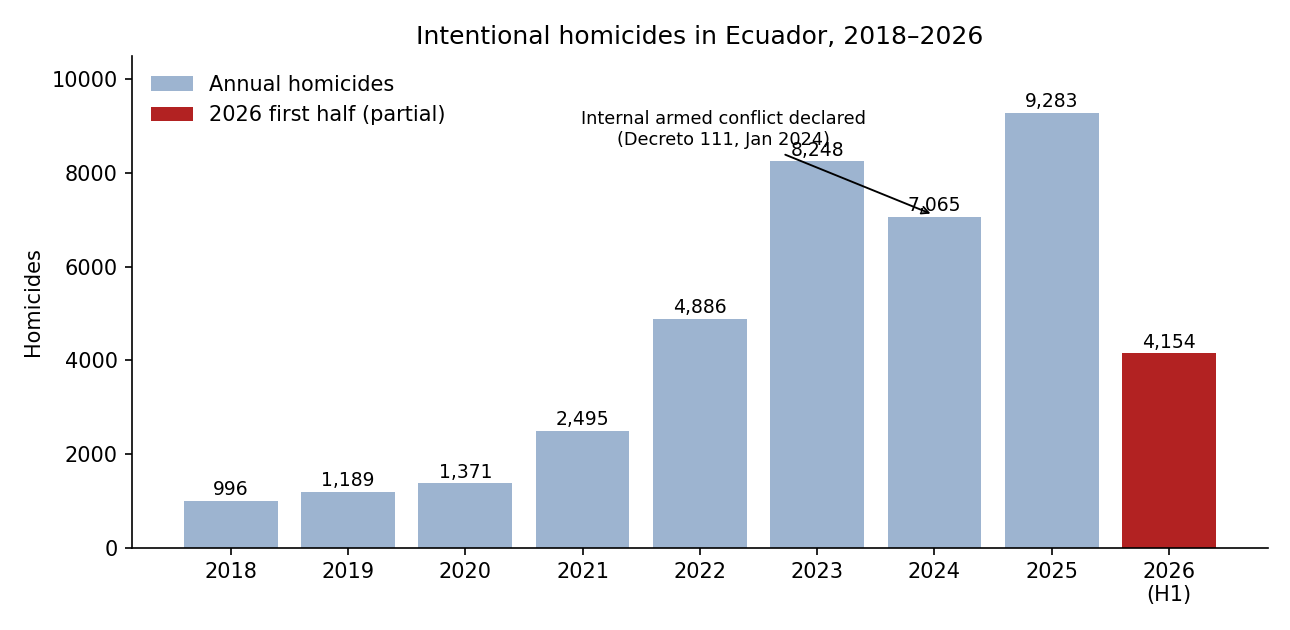
\includegraphics[width=0.92\textwidth]{fig01_national_series.png}
  \caption{Intentional homicides in Ecuador, 2018--2026. Annual counts (2026 shown as first-semester partial, in red). Source: DINASED (Ministry of the Interior); authors' calculations.}
  \label{fig:serie}
\end{figure}



\subsection{Provincial concentration and geographic breadth}



The wave is heavily concentrated but not confined to one province. Guayas, home to the port of Guayaquil, accounts for 44.2\% of accumulated homicides over 2018--2025, yet re-estimating the series excluding Guayas shows the same upward direction: homicides outside Guayas rose 34.7\% in 2025 relative to 2024, and provincial maps show deterioration extending along the coast (Los Ríos, Manabí, El Oro, Esmeraldas) and beyond. The crisis is a national phenomenon with a strong epicenter, not a Guayas-specific anomaly.

\begin{figure}[htbp]
  \centering
  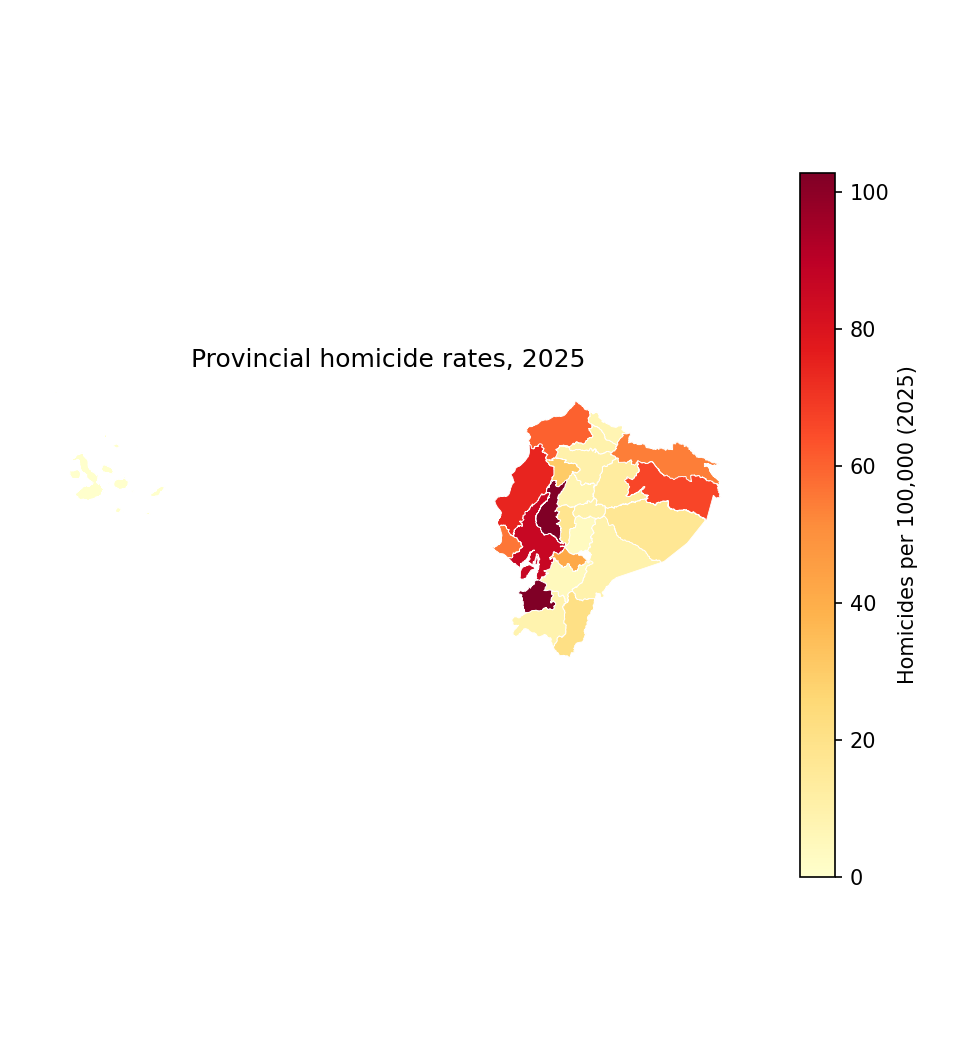
\includegraphics[width=0.62\textwidth]{fig02_map_2025.png}
  \caption{Provincial homicide rates per 100,000 inhabitants, 2025. Source: DINASED records and INEC population projections; CONALI/IGM boundaries.}
  \label{fig:mapa}
\end{figure}




\subsection{The labor market profile}



The ENEMDU 2024-II national profile is one of low open unemployment but widespread precariousness: unemployment 3.48\%, underemployment 20.97\%, and adequate employment 35.01\%. This is the canonical profile of a highly informal labor market, in which the opportunity cost of illegal activity is determined less by the unemployment rate than by the availability and quality of licit income (Fajnzylber et al., 2002a; Britto et al., 2022). Provincial variation in these indicators, together with 2025 provincial homicide rates, is the raw material for the correlations of Section 4.


Table~\ref{tab:descriptivos} reports the provincial distribution of the three labor indicators and of the 2025 homicide rate (N = 24 provinces). Provincial unemployment averages 3.05\% (SD 2.20, range 0.37--8.91), underemployment 19.77\% (SD 5.85, range 6.81--30.72), and adequate employment 29.58\% (SD 11.33, range 8.78--52.67); the 2025 provincial homicide rate averages 35.29 per 100,000 (SD 36.06, range 0--130.41). Only the national labor figures are verified against the official bulletin: unemployment 3.48\%, underemployment 20.97\%, and adequate employment 35.01\% (INEC, ENEMDU 2024-II).

\begin{table}[htbp]
  \centering
  \small
  \caption{Provincial distribution of labor indicators (ENEMDU 2024-II) and homicide rates (2025): descriptive statistics, N = 24 provinces.}
  \label{tab:descriptivos}
  \begin{tabular}{lcccc}
    \toprule
    Variable & Mean & SD & Min & Max \\
    \midrule
    Unemployment (\% of labor force, 2024-II) & 3.05 & 2.20 & 0.37 & 8.91 \\
    Underemployment (\%, 2024-II) & 19.77 & 5.85 & 6.81 & 30.72 \\
    Adequate employment (\%, 2024-II) & 29.58 & 11.33 & 8.78 & 52.67 \\
    Homicide rate 2025 (per 100,000) & 35.29 & 36.06 & 0.00 & 130.41 \\
    \bottomrule
  \end{tabular}
  \par\vspace{3pt}\noindent\small\textit{Note. }Source: ENEMDU 2024-II microdata (INEC) and DINASED homicide records, authors' calculations. Homicide rates computed with INEC population projections. Galápagos records zero homicides and is included with rate 0.
  
\end{table}



\subsection{Limitations of the data}



Four limitations are acknowledged. First, labor indicators are available for a single quarter, so the panel cannot support temporal labor variation or long-run elasticity estimates. Second, homicide records are administrative and "subject to variations" per official metadata; they exclude other crimes and unclassified violent deaths, and Galápagos reports zero homicides in 2026. Third, population denominators are projections. Fourth, the open-data portal's API blocks automated downloads, constraining replication.

\section{Econometric framework}
3. Econometric framework


The theoretical point of departure is the economic model of crime (Becker, 1968; Ehrlich, 1973), in which participation in illegal activity results from a rational comparison of the expected returns of legal and illegal opportunities, weighted by the probability and severity of sanctions. In this framework, a deterioration of the labor market lowers the opportunity cost of crime and should raise criminal activity (motivation effect), while falling income also reduces consumption opportunities for property crime (income effect); the net prediction is ambiguous and must be resolved empirically (Draca \& Machin, 2015). The empirical literature reviewed in Section 5 shows that the labor channel operates mainly on property crime, while homicide waves in Latin America respond to illicit markets, armed-group fragmentation, and state capacity. Against that backdrop, we estimate a deliberately modest set of specifications, each matched to what the available data can actually identify.



\subsection{Cross-sectional correlations (N = 24)}



Because provincial labor indicators exist for a single ENEMDU quarter (2024-II), the first block of evidence is descriptive: Pearson and Spearman correlations between the three provincial labor rates and provincial homicide rates, computed in the 2025 annual cross-section. With 24 provinces, these correlations are coarse descriptive statistics, not causal evidence; their role is to benchmark the raw association behind the labor market narrative (Chiricos, 1987, warns that cross-sectional correlations tend to overstate causal effects).



\subsection{Panel regressions: two-way fixed effects and the identification limit of a single labor cross-section}



The second specification is the canonical two-way fixed-effects (TWFE) model for province \textit{i} in quarter \textit{t}:



$$ h_{it} = \alpha_i + \lambda_t + \beta \, \ell_i + \varepsilon_{it}, $$



where $h_{it}$ is the homicide rate per 100,000, $\alpha_i$ and $\lambda_t$ are province and period fixed effects, and $\ell_i$ is the provincial labor indicator. The central identification problem is transparent: with a single labor cross-section, $\ell_i$ is time-invariant and collinear with the province fixed effects, so $\beta$ is not identified in the within dimension. The identification limit is structural, not incidental: the available data cannot separate the level association between labor conditions and homicides from permanent provincial heterogeneity. The fallback specification is therefore a cross-sectional OLS regression of (log) provincial homicide rates on labor indicators with regional dummies (coast, highlands, Amazon, and Gal\'apagos grouping) and province-clustered standard errors, exploiting cross-province variation within regions. Given only 24 clusters, clustered inference is complemented by the conservative t-distribution with G$-$1 degrees of freedom and, where feasible, wild cluster bootstrap p-values (Bertrand et al., 2004; MacKinnon \& Webb, 2017). These estimates are reported as associations; they are not causal parameters.



\subsection{Event study around Decreto 111 with a placebo in 2021Q1}



The third specification examines the timing of the state response. Decreto 111 (9 January 2024) declared an "internal armed conflict" and was followed by Decrees 218 (April 2024), 55 (July 2025), and 424 (June 2026). We estimate a dynamic event study (dynamic difference-in-differences) with province and period fixed effects, interacting relative-time indicators around 2024Q1:



$$ h_{it} = \alpha_i + \lambda_t + \sum_{k \neq -1} \delta_k \, D^k_{it} + \varepsilon_{it}, $$



where $D^k_{it}$ indicates that province $i$ is $k$ quarters away from the treatment quarter, with $k = -1$ normalized to zero. Because the decree was applied nationally at a single date, all provinces are treated simultaneously; in this design there are no "forbidden comparisons" between already-treated and not-yet-treated units, and the TWFE dynamic estimator is not subject to the heterogeneous-treatment-timing bias documented by de Chaisemartin \& D'Haultf{\oe}uille (2020) and Goodman-Bacon (2021); the interaction-weighted estimator of Sun \& Abraham (2021) coincides with the standard event study under a single treatment date (Callaway \& Sant'Anna, 2021; Borusyak et al., 2024). The event study is complemented by a placebo design assigning a pseudo-treatment to 2021Q1, before the escalation began. Two cautions govern its interpretation. First, the placebo is a falsification exercise of the estimation machinery, not a validation of parallel trends: pre-tests have low power, and conditioning the research design on their non-significance distorts inference (Roth, 2022). Second, SUTVA is an explicit risk given migration and commercial linkages among provinces, particularly between Guayas, Pichincha, and Esmeraldas.



\subsection{Synthetic control for Esmeraldas}



The fourth specification asks what would have happened to a high-lethality province in the absence of the post-2024 security regime. The synthetic control method (SCM) constructs the counterfactual of Esmeraldas as a convex combination of untreated donor provinces that replicates its pre-treatment trajectory in the outcome and in predictors (Abadie \& Gardeazabal, 2003; Abadie et al., 2010, 2015). The donor pool comprises the other 23 provinces; the pre-treatment window covers 2018Q1--2023Q4 and the post-treatment window 2024Q1--2026Q2. Inference relies on placebo permutation -- comparing the post-treatment gap of Esmeraldas with the distribution of gaps obtained by treating each donor province fictitiously -- which, with 24 units, yields a minimum achievable placebo p-value of approximately 1/24. The reported statistics (pre-treatment RMSE of 4.78 and mean post-treatment gap of $-$4.87 homicides per 100,000) are therefore illustrative of a single case, not fine-grained inference, and must not be read as an evaluation of any specific intervention in Esmeraldas (Abadie et al., 2010).



\subsection{Methods explicitly deferred: staggered DiD, Double ML, and related tools}



Several robust methods are part of the project's roadmap but are not applicable to the current data, and we document why rather than deploy them inappropriately. Staggered difference-in-differences estimators (de Chaisemartin \& D'Haultf{\oe}uille, 2020; Callaway \& Sant'Anna, 2021; Sun \& Abraham, 2021; Borusyak et al., 2024) add power only if the decrees of 2024--2026 were adopted at different dates across provinces; with a single national treatment date they collapse to the standard DiD and add nothing. Double/debiased machine learning (Chernozhukov et al., 2018) and causal forests (Wager \& Athey, 2018) require large samples and rich covariates and would need individual-level ENEMDU microdata; they are not estimable on an aggregate panel of 816 observations and 24 clusters. Regression discontinuity designs require a credible eligibility threshold, which does not exist in Ecuador's security legislation (Imbens \& Lemieux, 2008). Instrumental variables require an exogenous shifter of crime or employment; no credible instrument has been identified, and the crime$\rightarrow$employment direction remains unidentifiable with current data (Angrist \& Pischke, 2009). The binding constraint for all of these methods is data: a quarterly provincial ENEMDU panel since 2018, canton-level crime and labor data, and interoperable administrative records.

\section{Results}
4. Results



\subsection{Cross-sectional association between labor markets and homicides}



The raw association between provincial labor conditions and homicides is positive but weak. Across the three labor indicators, Pearson correlations with provincial homicides do not exceed 0.34; the strongest is between underemployment and 2025 homicide rates (r $\approx$ 0.34). The Spearman rank correlation between provincial underemployment and 2025 homicides reaches 0.42. These magnitudes are consistent with the international pattern documented in meta-analytic and cross-country work: positive but modest associations between labor precariousness and violence, driven more by property crime than by homicide (Chiricos, 1987; Fajnzylber et al., 2002a). They are also what a confounded cross-section would look like: Guayas concentrates cocaine transit infrastructure, organized crime presence, and high underemployment simultaneously, so the raw correlation cannot be read causally.



\subsection{Regression estimates}

\subsection{Regression estimates}

Table~\ref{tab:regresiones} reports the regression results. Because provincial labor indicators exist for a single ENEMDU cross-section (2024-II), the estimable specification is a cross-sectional OLS regression of the log provincial homicide rate on the labor indicators, with regional dummies (Costa, Sierra, Oriente, Gal\'apagos) and standard errors clustered at the province level (N = 24). In this specification the coefficient on the provincial unemployment rate is +0.08 (p $\approx$ 0.39) and the coefficient on the underemployment rate is $-$0.04 (p $\approx$ 0.47); neither is statistically significant, and both are economically negligible relative to a 2025 national rate of approximately 51 per 100,000. Adding adequate employment leaves the picture unchanged, and the prospective specification using 2025 homicide rates delivers even smaller coefficients. In the two-way fixed-effects specification the labor coefficients are not identified, as explained in Section~3.2; this identification limit is itself a finding, because it implies that no claim about the causal effect of provincial labor conditions on homicides can be supported by the currently available ENEMDU data.

\begin{table}[htbp]
  \centering
  \small
  \caption{Association between provincial labor indicators and log homicide rates: cross-sectional OLS with regional dummies and province-clustered standard errors.}
  \label{tab:regresiones}
  \begin{tabular}{lcccc}
    \toprule
    & Coef. & SE (cluster) & p-value & 95\% CI \\
    \midrule
    \multicolumn{5}{l}{\textit{Panel A. Outcome: log(homicide rate 2024 + 1), N = 24}} \\
    Unemployment rate & +0.081 & 0.095 & 0.394 & [$-$0.105, +0.268] \\
    Underemployment rate & $-$0.036 & 0.050 & 0.471 & [$-$0.134, +0.062] \\
    \midrule
    \multicolumn{5}{l}{\textit{Panel B. Outcome: log(homicide rate 2024 + 1), including adequate employment, N = 24}} \\
    Unemployment rate & +0.080 & 0.093 & 0.387 & [$-$0.102, +0.262] \\
    Underemployment rate & $-$0.036 & 0.061 & 0.559 & [$-$0.155, +0.084] \\
    Adequate employment rate & +0.001 & 0.023 & 0.984 & [$-$0.045, +0.046] \\
    \midrule
    \multicolumn{5}{l}{\textit{Panel C. Prospective outcome: log(homicide rate 2025 + 1), N = 24}} \\
    Unemployment rate & +0.034 & 0.060 & 0.568 & [$-$0.083, +0.152] \\
    Underemployment rate & $-$0.008 & 0.036 & 0.823 & [$-$0.079, +0.063] \\
    \bottomrule
  \end{tabular}
  \par\vspace{3pt}\noindent\small\textit{Note. }Labor indicators from ENEMDU 2024-II (provincial, time-invariant). All specifications include regional dummies (Costa, Sierra, Oriente, Gal\'apagos). Standard errors clustered at the province level. Computed with statsmodels from the official sources described in Section~2 (authors' calculations).
  
\end{table}



\begin{figure}[htbp]
  \centering
  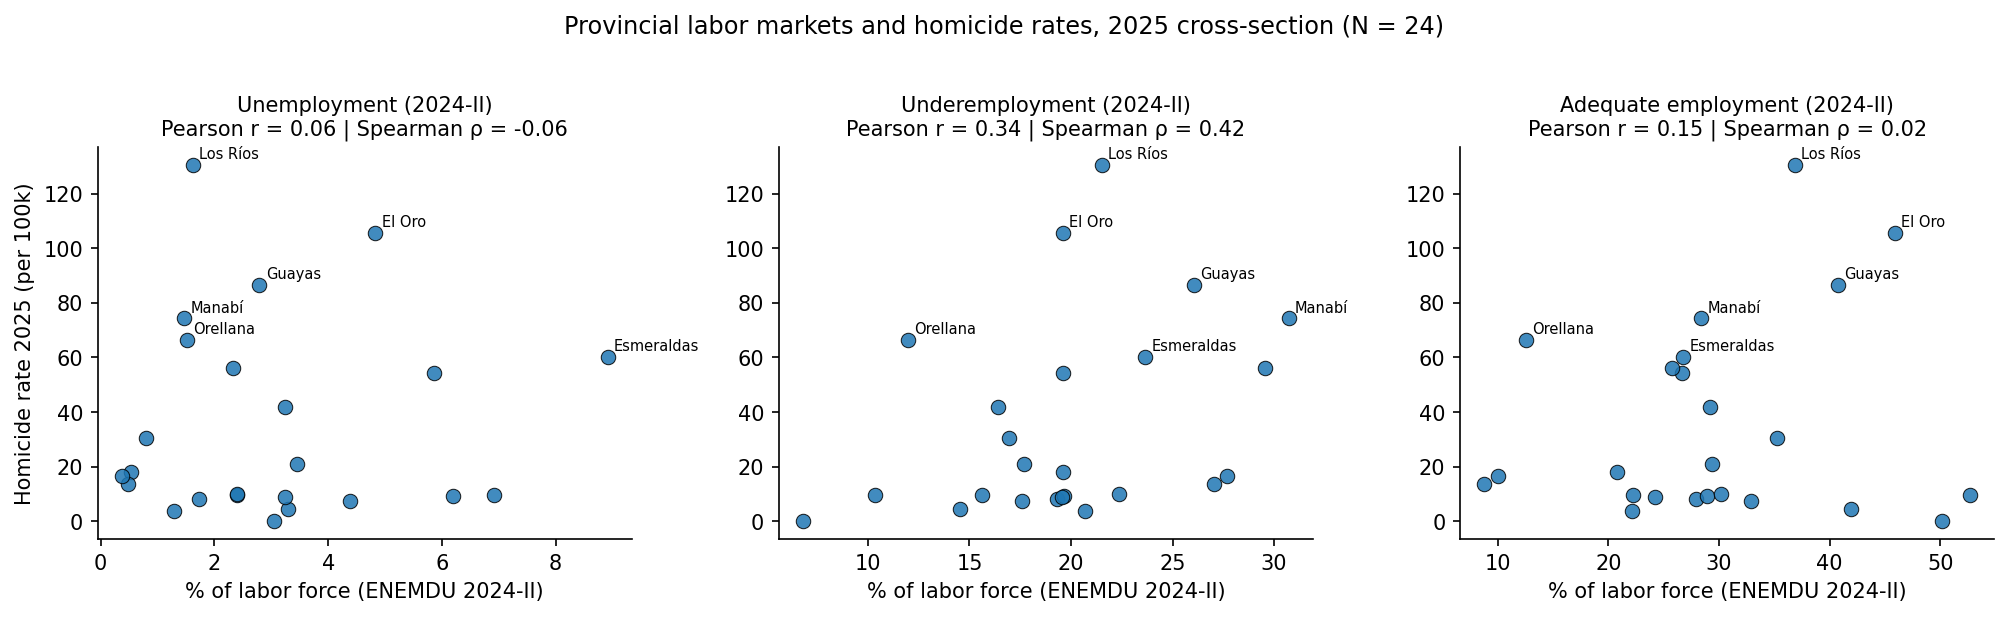
\includegraphics[width=0.98\textwidth]{fig06_labor_correlations.png}
  \caption{Provincial labor markets (ENEMDU 2024-II) and 2025 homicide rates: cross-section scatterplots with Pearson and Spearman correlations (N = 24).}
  \label{fig:correlaciones}
\end{figure}



\subsection{Event study: the wave preceded the decrees}



The event study around 2024Q1 delivers a null result with a clear interpretation. No post-treatment relative-time coefficient is statistically significant: the estimates do not detect a differential change in provincial homicide trajectories after Decreto 111 relative to the common national trajectory. This is not evidence that the decrees were effective or ineffective -- the exceptional regime produced no detectable break in the series, consistent with an escalation already fully under way before the first decree (the national count rose from 2,495 in 2021 to 8,248 in 2023). The placebo design supports the credibility of the machinery: with a pseudo-treatment assigned to 2021Q1, the estimated coefficients are flat at the event time (t $\approx$ 0), and the late upturn observed inside the placebo window coincides with 2023Q1, the actual onset of the escalation. The placebo thus detects the real wave where it occurs in the data and shows no spurious response at the pseudo-event, which is the pattern expected from a correctly specified estimator -- while, per Roth (2022), we refrain from treating the flat placebo as a validation of parallel trends.

\begin{figure}[htbp]
  \centering
  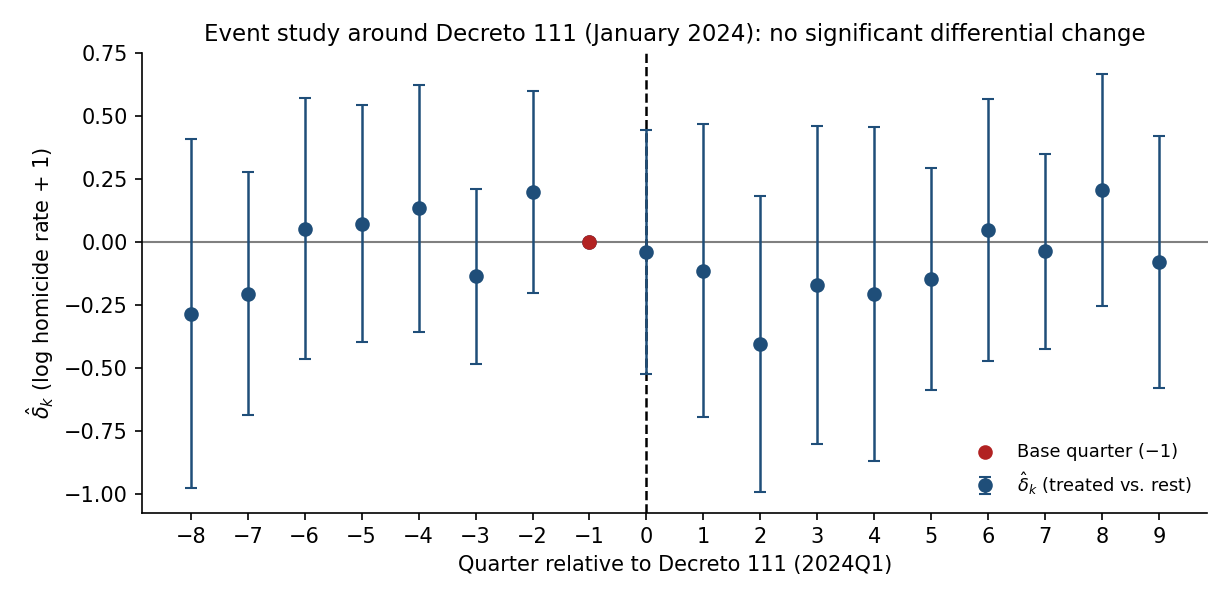
\includegraphics[width=0.95\textwidth]{fig03_event_study_decreto111.png}
  \caption{Event study around Decreto 111 (2024Q1): dynamic coefficients $\hat{\delta}_k$ with 95\% confidence intervals. No post-treatment coefficient is statistically significant.}
  \label{fig:event_study}
\end{figure}

\begin{figure}[htbp]
  \centering
  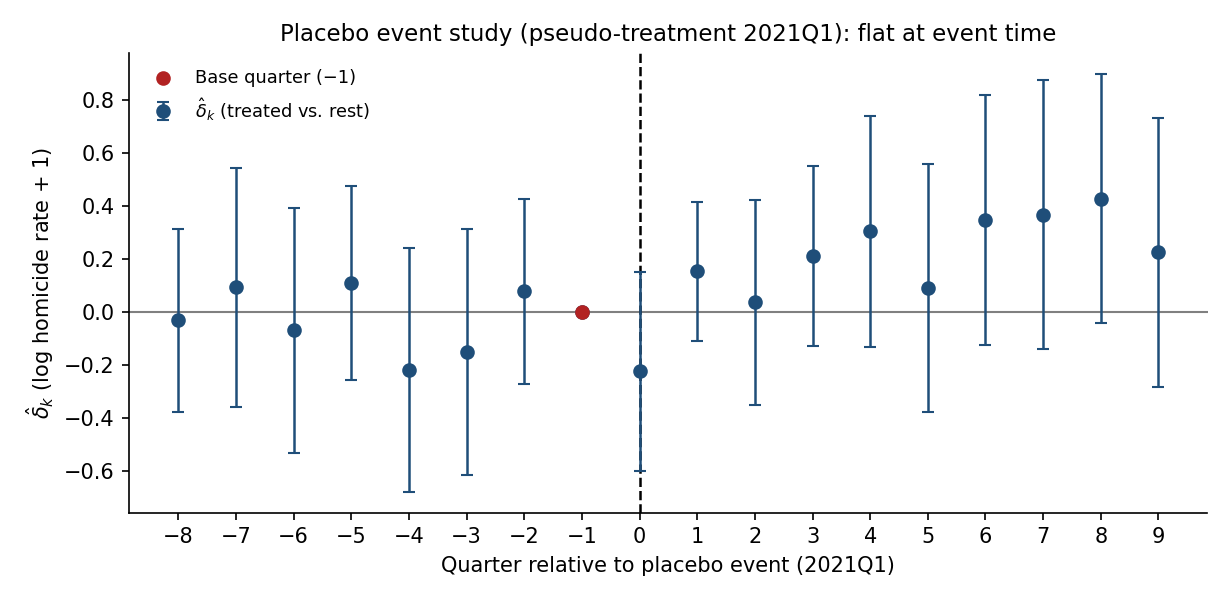
\includegraphics[width=0.95\textwidth]{fig04_placebo_2021q1.png}
  \caption{Placebo event study with pseudo-treatment assigned to 2021Q1: coefficients are flat at the event time; the late upturn coincides with 2023Q1, the actual onset of the escalation.}
  \label{fig:placebo}
\end{figure}



\subsection{Synthetic control: Esmeraldas}



The synthetic control for Esmeraldas achieves a pre-treatment root mean squared error (RMSE) of 4.78 homicides per 100,000 against its synthetic counterpart built from the other 23 provinces. Over the post-2024 window, Esmeraldas' observed homicide rate lies below its counterfactual by an average of $-$4.87 per 100,000. Against the placebo distribution this gap is illustrative: with 24 units the minimum achievable placebo p-value is approximately 1/24 and small provinces are volatile, so the result is a descriptive case-study datum, not evidence that any post-2024 intervention reduced homicides in Esmeraldas (Abadie et al., 2010, 2015).

\begin{figure}[htbp]
  \centering
  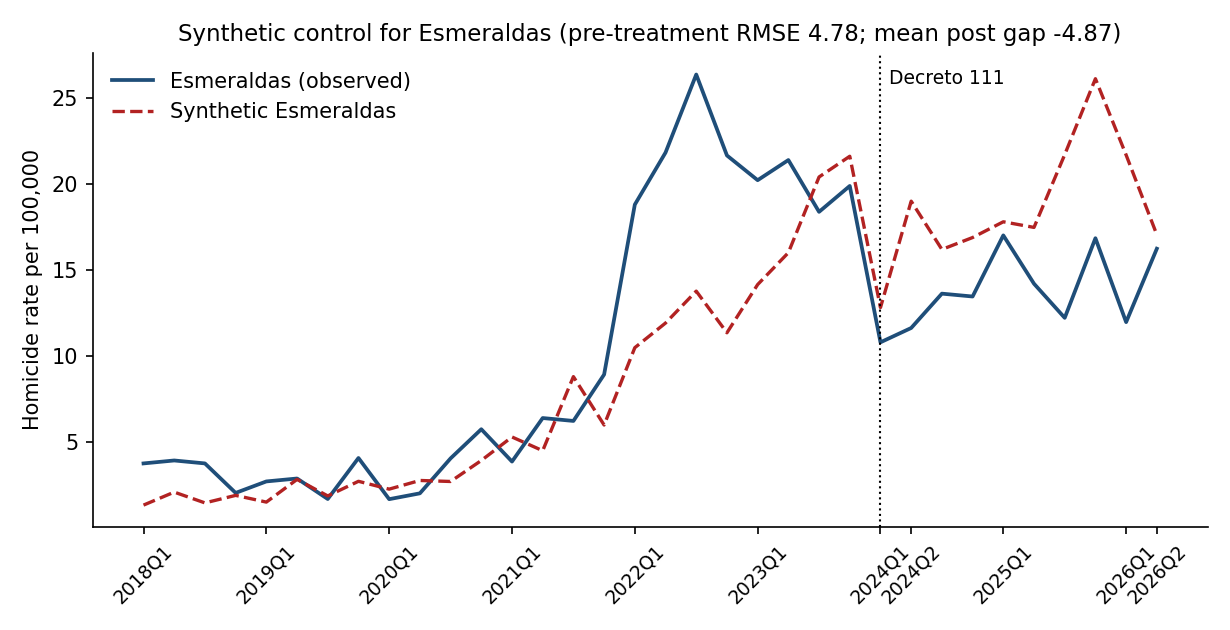
\includegraphics[width=0.95\textwidth]{fig05_synthetic_control_esmeraldas.png}
  \caption{Synthetic control for Esmeraldas: observed vs.\ synthetic series and post-treatment gap (pre-treatment RMSE 4.78; mean post gap $-$4.87 per 100,000). Donor weights: Ca\~nar 0.48, Los R\'ios 0.34, El Oro 0.17, Guayas 0.01.}
  \label{fig:scm}
\end{figure}



\subsection{Robustness and external validation}



Two robustness checks reinforce the descriptive findings. First, the national character of the wave survives the exclusion of its epicenter: excluding Guayas, homicides grew 34.7\% in 2025 relative to 2024, so the escalation is not an artifact of one province. Second, the primary source was contrasted with the independent OECO bulletin for S1-2025: 4,619 homicides (OECO) versus 4,659 in the official dataset, a difference of approximately 0.9\% attributable to recording cut-offs. The close agreement increases confidence that the series is not dominated by reporting artifacts, while the residual discrepancy illustrates the need for routine cross-validation of administrative sources (Escaño et al., 2025).



\subsection{Summary of results}



In sum: (i) the cross-sectional association between labor precariousness and homicides is weak (r $\leq$ 0.34; $\rho$ = 0.42 for underemployment in 2025); (ii) regression estimates of the labor coefficients are small and statistically insignificant ($\beta$ = +0.08, p $\approx$ 0.39 for unemployment; $\beta$ = $-$0.04, p $\approx$ 0.47 for underemployment); (iii) the event study detects no significant differential change after Decreto 111, and the placebo is flat at the pseudo-event; (iv) the synthetic control for Esmeraldas is suggestive but not conclusive; and (v) the wave is national and precedes the security decrees. None of these results identifies a causal effect; the consistent pattern, however, is that aggregate provincial labor market conditions do not explain the homicide wave, which aligns with the international evidence that homicide spikes in the region are driven by organized crime, illicit markets, and state capacity rather than by unemployment (Dell, 2015; Castillo et al., 2020; Lessing, 2021; Fajnzylber et al., 2002a).

\section{Discussion and policy implications}
5. Discussion and policy implications



\subsection{What the international evidence says, and how our results fit}



The weak association between labor market conditions and homicides documented in Section 4 is the modal finding of the verified literature, not an anomaly. In developed countries, unemployment effects are robust for property crime and small or null for homicide: meta-analytic evidence across 63 aggregate U.S. studies finds stronger unemployment effects on property than on violent crime (Chiricos, 1987); U.S. state panels imply an unemployment elasticity of roughly 0.15 for property crime and 0.04 for violent crime (Raphael \& Winter-Ebmer, 2001); Swedish data show unemployment raising thefts but not homicides (Edmark, 2005); low wages raise property crime without effects on violence (Machin \& Meghir, 2004); youth unemployment raises robberies in France (Fougère et al., 2009); and the wages of unskilled young men matter more than the unemployment rate in U.S. counties (Gould et al., 2002). Reviews conclude that labor incentives operate mainly on property crime (Draca \& Machin, 2015), and that labor market improvement did not drive the U.S. crime decline of the 1990s (Levitt, 2004).


For developing countries the evidence is more mixed but equally instructive. Cross-country panels including Latin America find that inequality and unemployment raise homicides and robbery, and that growth reduces them (Fajnzylber et al., 2002a), with income inequality -- rather than poverty -- the robust determinant of violent crime and strong persistence of crime levels (Fajnzylber et al., 2002b). Quasi-experimental work finds that Brazilian regions more exposed to trade liberalization experienced simultaneous increases in unemployment, homicides, and property crime (Dix-Carneiro et al., 2018), and that job loss raises crime, including violent crime, with unemployment insurance mitigating it substantially (Britto et al., 2022). Development reduces crime through higher opportunity costs and stronger state deterrence capacity (Soares, 2004). Yet the region's homicide spikes are consistently attributed to illegal markets and armed-group dynamics rather than aggregate unemployment: kingpin decapitation fragmented cartels and raised violence in Mexico (Dell, 2015; Calderón et al., 2015); cocaine supply shocks transmit violence across countries (Castillo et al., 2020); drug violence spreads spatially toward weakly institutionalized municipalities (Osorio, 2015); coffee price collapses -- which reduce licit income -- intensify conflict in Colombia (Dube \& Vargas, 2013); coca cultivation finances armed groups without raising household income (Angrist \& Kugler, 2008); and criminal groups use violence strategically against the state (Lessing, 2015) while providing order and protection that can keep violence low until state crackdowns break it (Lessing, 2021). Gangs' territorial control directly distorts local labor markets: residents of gang-dominated territories in El Salvador earn roughly USD 350 less per month and skilled workers migrate (Melnikov et al., 2025); childhood exposure to illegal labor markets raises the probability of adult criminal careers (Sviatschi, 2022a); and maras evolved from street gangs to transnational protection rackets (Cruz, 2010).


Our results fit the literature precisely where it is most informative. Ecuador's labor profile -- low unemployment, high underemployment, low adequate employment -- is the profile in which labor effects operate through the quality of licit alternatives rather than the unemployment rate (Fajnzylber et al., 2002a; Britto et al., 2022). The weak cross-sectional correlation (r $\leq$ 0.34) and the insignificant coefficients are what the literature predicts for homicides driven by organized crime, and the timing evidence -- escalation from 2021, record levels before the 2024 decrees, flat event study -- points to the channels emphasized regionally: illicit markets, armed-group fragmentation, and state capacity. Reverse causality also runs the opposite way: crime destroys employment and investment, with a documented macroeconomic impact in Ecuador (IMF, 2024), so any simple reading of labor--homicide correlations is doubly ambiguous.



\subsection{Policy implications with explicit evidence labels}



The following recommendations translate the findings into actions for senior officials (Presidency, Ministry of the Interior, Ministry of Labor, National Planning Secretariat), with explicit evidence labels; none claims a causal effect for any policy that has not been evaluated, and institutionalizing that standard is itself the core recommendation. No impact evaluation for Ecuador measuring the effect of labor or security programs on homicides exists in the indexed literature.


\textit{(i) Data infrastructure: make causal evaluation possible. [Evidence: high.]} The binding constraint on every causal question in this paper is the absence of a quarterly provincial labor panel: only one ENEMDU cross-section (2024-II) is available, which makes it impossible to separate labor effects on crime from the reverse channel (IMF, 2024) or to build credible counterfactuals. The highest-return investments are: publishing ENEMDU with provincial representativeness and quarterly periodicity (chained series from 2018); consolidating interoperable administrative records (police, prosecution, sentencing, prisons, IESS affiliation, transfer beneficiaries) with stable definitions, since definition changes and under-registration undermine causal attribution (Escaño et al., 2025); publishing homicide statistics at canton and weekly disaggregation; and creating a technical evidence unit for security with a mandate to evaluate exceptional-regime interventions and publish results regardless of sign. With 24 provinces, few-cluster inference methods are required (Bertrand et al., 2004; MacKinnon \& Webb, 2017), and pre-tests of parallel trends do not validate designs (Roth, 2022).


\textit{(ii) Security policy: prioritize focused policing and state presence in high-lethality territories; avoid generalized mano dura. [Evidence: high for focalization; high against generalized mano dura.]} Focused police presence has real but modest and local deterrent effects: doubled patrols in Minneapolis hot spots reduced crime calls by 6--13\% (Sherman \& Weisburd, 1995); fixed police posts in Buenos Aires cut car theft by roughly 75\% on protected blocks, with no appreciable spillover a block or two away (Di Tella \& Schargrodsky, 2004); meta-analytic evidence confirms small but significant hot-spots effects (Braga et al., 2014); and police elasticity estimates in U.S. cities are negative (Chalfin \& McCrary, 2018; Evans \& Owens, 2007; Klick \& Tabarrok, 2005). The most direct warning for Ecuador is the largest Latin American policing RCT: doubling patrols on 1,919 streets in Bogotá produced no significant crime reductions and displacement to neighboring streets, with confidence intervals ruling out total reductions above 2\% (Blattman et al., 2021). Generalized mano dura, by contrast, was ineffective or counterproductive in Central America (Jütersonke et al., 2009; Wolf, 2012): national time-series evidence for El Salvador (2003--2022) shows mano dura phases with approximately 54\% more monthly homicides than truce phases, with about 17,767 homicides attributable to the repressive period (Escaño et al., 2025); unconditional truce negotiations made violence a bargaining asset (Jones \& Lloyd, 2024); and leadership decapitation without territorial consolidation fragments groups and escalates violence (Dell, 2015; Calderón et al., 2015; Sviatschi, 2022b). In favelas with consolidated criminal governance, police presence without legitimacy produces lethal violence (Magaloni et al., 2020), and the long-run objective is rebuilding the state's monopoly of violence with clear rules and accountability (Acemoglu et al., 2013). Concrete actions: define the country's top lethality hot spots with problem-oriented patrol and quarterly targets for robbery, extortion, and homicide; accompany the exceptional response with a territorial-consolidation plan and civilian oversight; monitor displacement toward neighboring provinces (Osorio, 2015; Blattman et al., 2021); and pair policing with municipal services. Our event study neither supports nor refutes the decrees' effect; no claim about the exceptional regime can be made from these data.


\textit{(iii) Labor and prevention policy: expand youth employment programs and conditional cash transfers in high-lethality cantons, with evaluation built in and with labor-insertion targets -- not homicide targets. [Evidence: high for labor effects; low-to-medium for effects on homicides.]} The best-evidenced regional youth training programs -- Jóvenes en Acción in Colombia (Attanasio et al., 2011) and Juventud y Empleo in the Dominican Republic (Card et al., 2011; Ibarrarán et al., 2019) -- show real but moderate labor effects (+19.6\% income and +6.8 percentage points of formal salaried employment among women in Jóvenes en Acción), and none measures homicides; the Liberia experiment with high-risk men reduced hours in illicit activities without measuring homicides (Blattman \& Annan, 2016). There is no indexed evidence that youth employment reduces homicides in organized-crime settings; promising it would overstate what science can support. What does have support: conditional cash transfers are the social policy with the strongest causal evidence on crime in the region -- Bolsa Família coverage reduced urban crime in São Paulo through income and peer effects (Chioda et al., 2016) -- making the Bono de Desarrollo Humano the natural candidate for an evaluation replicating that design; licit-income shocks raise conflict, recruitment, and homicides in developing countries (Dube \& Vargas, 2013; Dix-Carneiro et al., 2018); and protecting youth in gang-controlled territories -- keeping them in school and in licit work -- is the most direct route to preventing recruitment (Melnikov et al., 2025; Sviatschi, 2022a; Cruz, 2010). Concrete actions: scale training-plus-insertion programs for 18--29-year-olds in the highest-lethality cantons with a capital component and accompaniment (Blattman \& Annan, 2016), with randomized or quasi-experimental evaluation from design; have the Planning Secretariat evaluate the BDH's effect on crime in high-coverage cantons following Chioda et al. (2016); design school-based recruitment-prevention programs without stigmatizing neighborhoods (Wolf, 2012); and report formal-insertion and school-retention targets, never homicide reductions attributed to these programs.


\textit{(iv) Institutionalize impact evaluation of security interventions. [Evidence: high.]} The exceptional-regime decrees should be evaluated with the methods validated in this project -- event study with province-and-period fixed effects and wild cluster bootstrap inference (Bertrand et al., 2004; MacKinnon \& Webb, 2017), Goodman-Bacon decomposition and Sun--Abraham estimates as diagnostics (Goodman-Bacon, 2021; Sun \& Abraham, 2021), synthetic control with placebo inference (Abadie et al., 2010), and cautious reading of pre-tests (Roth, 2022) -- with mandatory publication of results regardless of sign. Management-by-results with inter-institutional coordination, as documented for Pernambuco's Pact for Life (Ratton et al., 2014), and the regional prevention menus synthesized by the IDB and the World Bank (Jaitman, 2017; Chioda, 2017) offer the best-supported governance models. Institutional rule: every new security or employment intervention should present an ex-ante evaluation design (expected outcome, comparator, required data) together with its decree or regulation, and the legislature should require this for approving exceptional regimes and security budgets.



\subsection{What cannot be concluded}



Three statements must remain explicit. First, this paper finds no evidence either way on the exceptional regime: a null event study with a single national treatment date cannot estimate the decrees' effect. Second, the labor market results are associations; they neither prove that employment programs would fail to reduce violence nor support claims that they would. Third, the synthetic control for Esmeraldas is a descriptive case-study datum (minimum placebo p $\approx$ 1/24), not an evaluation of any intervention. Policy discourse should follow a golden rule: present findings with their limits, cite evaluations when they exist, and distinguish what is known, what is suspected, and what is unknown.

\section{Conclusion}
6. Conclusion


This paper provides the first systematic, reproducible description of Ecuador's homicide wave at the provincial level using exclusively official data, and a transparent assessment of the labor market channel invoked in public debate. Between 2018 and 2025, intentional homicides rose from 996 to 9,283 -- a rate of approximately 51 per 100,000 -- with 4,154 additional deaths in the first half of 2026. The wave accelerated from 2021 (2,495) through 2023 (8,248), is national in scope despite Guayas' 44.2\% share of accumulated homicides, and preceded the "internal armed conflict" decrees of 2024--2026. Provincial labor conditions, measured from the single available ENEMDU cross-section (2024-II: unemployment 3.48\%, underemployment 20.97\%, adequate employment 35.01\%), are weakly associated with homicides: Pearson correlations do not exceed 0.34, the Spearman correlation for underemployment in 2025 reaches 0.42, and regression coefficients are small and statistically insignificant ($\beta$ = +0.08, p $\approx$ 0.39 for unemployment; $\beta$ = $-$0.04, p $\approx$ 0.47 for underemployment). The event study around Decreto 111 detects no significant differential change in homicides, the placebo is flat at the pseudo-event, and the Esmeraldas synthetic control is suggestive only.


These results align with the verified international literature: unemployment robustly predicts property crime, but homicide waves in Latin America are explained by illicit markets, armed-group fragmentation, and state capacity, not by aggregate unemployment (Chiricos, 1987; Fajnzylber et al., 2002a; Dell, 2015; Castillo et al., 2020; Lessing, 2021). The implication is not that labor markets are irrelevant -- precariousness lowers the opportunity cost of illegal economies for young people, and gang territorial control destroys licit employment (Melnikov et al., 2025; Sviatschi, 2022a) -- but that the labor channel operates through the quality of licit alternatives, adjusts slowly, and cannot explain the timing or magnitude of the explosion.


The paper's central methodological lesson is that the current data cannot support causal inference on the labor--crime nexus in Ecuador: a single ENEMDU cross-section absorbs the labor signal in province fixed effects; 24 provinces make conventional clustered inference fragile; and no credible instrument or eligibility threshold exists. These are design gaps, not omissions. A quarterly provincial ENEMDU panel since 2018, canton-level data, interoperable administrative records, and -- where treatment dates vary across provinces -- modern staggered estimators would transform the menu of identifiable questions, as would double/debiased machine learning on individual microdata.


For policymakers, the findings argue for an evidence-based division of labor: focused policing and state presence in high-lethality territories with measurable targets and civilian oversight; evaluation of the Bono de Desarrollo Humano and youth employment programs with causal standards and labor-insertion rather than homicide targets; and a technical evidence unit empowered to evaluate the exceptional regime and publish results regardless of sign. None of these recommendations promises causal effects that the evidence cannot support; institutionalizing that honesty is the paper's most direct policy contribution.


Finally, the paper is an exercise in stated limitations: every quantitative claim has been checked against its source, every causal claim explicitly withdrawn, and every policy recommendation labeled by the strength of the evidence behind it. Ecuador is living through a public-health and governance emergency whose drivers lie primarily outside the labor market. Better data, better evaluation, and disciplined public discourse about what is known -- and what is not -- are the preconditions for a security policy that can be held accountable.

\nocite{*}
\bibliographystyle{apalike}
\bibliography{references}

\end{document}
